\chapter{Wireless sensors networks}

Traditional sensor monitoring was implemented with basic sensors made up only by transducers connected by a wire to a centralized device, such as Arduino.
In WSNs instead, the sensors are connected wirelessly to a centralized device, which is usually a computer or a microcontroller, and they present many characteristics:
\begin{itemize}
   \item Intelligent
   \item Wireless
   \item Autonomous
   \item Capable of building a Network
\end{itemize}

\section{Deploying a WSN}

\begin{paracol}{2}
   

   Sensor deployed in a ``Sensing Field'' form a network made up ---one or more--- sink nodes and a set of sensor nodes.
   Each sensor produces a stream of data which may be preprocessed by the sensor itself before being eventually sent to a sink node.
   Sinks may not always be available, so the sensors may act as ``loggers'' and store data for future retrieval; since energy efficiency is a key factor, some \textbf{data aggregation} may be performed on the network to improve the efficiency.
   
   \switchcolumn
   \begin{figure}[htbp]
      \centering
      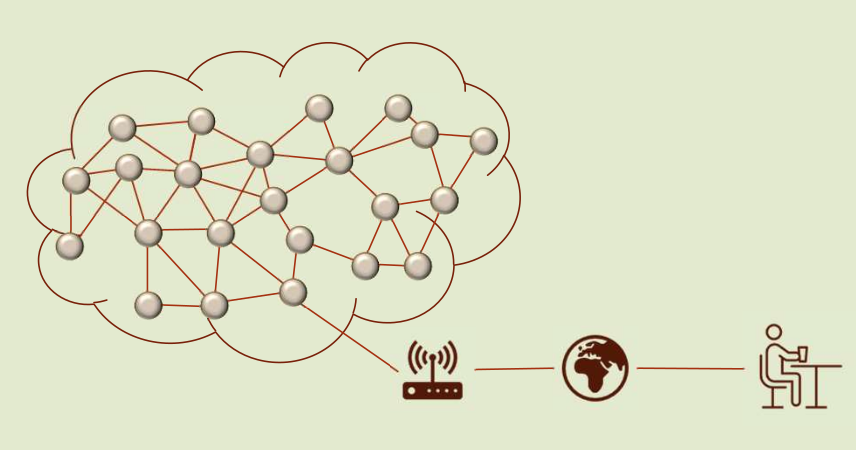
\includegraphics{images/wsn_arch.png}
      \caption{WSN architecture}
      \label{fig:wsn_arch}
   \end{figure}
\end{paracol}

\subsection{WSNs Strenghts}
\begin{itemize}
   \item Network deployment is easy:
   \begin{itemize}
      \item no need for cables
      \item self-configurable (no centralized control)
   \end{itemize}
   \item Sensors are cheap:
   \begin{itemize}
      \item The number of sensors can scale up
      \item redundant sensors to enforce fault tolerance
   \end{itemize}
   \item Sensors can be mobile
   \begin{itemize}
      \item if wearable or deployed on mobile objects
   \end{itemize}
   \item Sensors can be programmable on the fly
   \begin{itemize}
      \item to adapt to changing conditions
      \item to implement new sensing tasks
   \end{itemize}
\end{itemize}

\section{WSN Characteristics}
WSNs first of all may be data-centric or node-centric. This refers especially to routing algorithms, since tradinational ones are too resource-consuming for WSNs.
Most WSN are data-centric, meaning that the data is the most important thing, and the network is built around it.

\subsection{Implosion and Overlap}
The \textbf{``implosion''} problem happens due to flooding-based dissemination:
\begin{itemize}
   \item node A starts by flooding its data to all of its neighbors, including B,C connected to node D.
   \item Two copies of the data eventually arrive at
   the aggregation node D.
   \item The system wastes resources in one
   unnecessary send and receive.
\end{itemize}

The \textbf{``overlap''} problem happens when two nodes send the same data to the same node, which is a waste of resources. 
This may happen when to sensor cover the same overlapping geographical region. (e.g. two cameras covering the same area, or two termometers in the same room)

\subsection{Directed Diffusion}
This is an approach designed and presented by \textbf{Deborah Estrin} and her team in 2000 at Mobicom.

\begin{itemize}
   \item Data is \textbf{named} using attribute-value pairs.
   \item The sink disseminates a sensing task in the network as an interest for named data.
   \item The dissemination of interests sets up gradients.
   \item \note{gradients ``draw'' events (i.e. data matching the interest)}
   \item Data matching the interest flows towards the sink
   \note{Along the gradients, following multiple paths}
   \item The sink \textit{reinforces} one or some of these paths.
\end{itemize}
